\section{use case: investigation of the noise impact on Auto Encoder algorithm}

\subsection{Objective}
This section presents a complete case study that constructs artificial noise experiments to quantitatively evaluate the effects of three typical noise types—Gaussian noise, drift, and spikes—on the trajectory reconstruction performance of an autoencoder (AE) model. The results further help to identify key priorities and directions for the data cleaning stage.
The experiment employs an ADS-B dataset collected at Zurich Airport, covering trajectory data recorded from 04:57:13 (UTC) on October 1, 2019 to 18:57:37 (UTC) on November 30, 2019, as shown in Figure \ref{fig:totaltracks}. The dataset contains approximately 2.8 million ADS-B messages, representing the complete trajectories of about 14,000 flights. Each record includes fields such as timestamp, altitude, longitude, latitude, ground speed, heading, callsign, and ICAO24 code, with longitude ranging from 7.5702 to 9.5276 and latitude from 46.8019 to 48.1302.

% TODO: \usepackage{graphicx} required
\begin{figure}
	\centering
	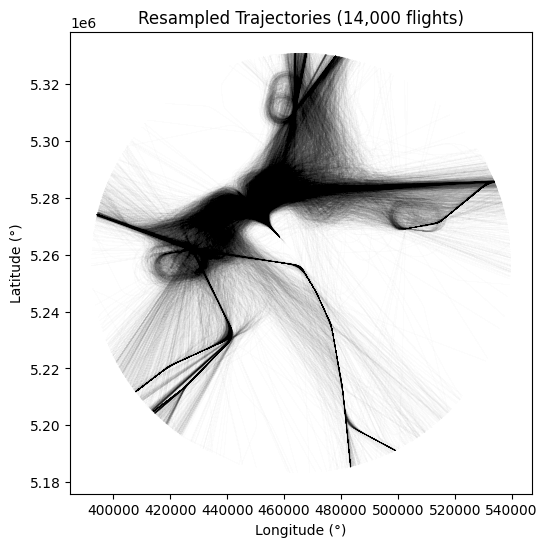
\includegraphics[width=0.7\linewidth]{totaltracks}
	\caption{Visualization of the whole dataset}
	\label{fig:totaltracks}
\end{figure}

For model training, the data were preprocessed as follows: trajectories were resampled so that each one contained 100 longitude–latitude coordinate points, ensuring a uniform input dimension; and normalization was applied to preserve the spatial proportion of coordinates.